% !TeX program = lualatex

\documentclass[aspectratio=169,xcolor={dvipsnames}
,hide notes
%,show only notes
%,show notes on second screen=right
]{beamer}
\usetheme[background=light, numbering=fraction]{metropolis}
\usepackage{appendixnumberbeamer}

%\usepackage[T1]{fontenc}

\usepackage{bm}

\usepackage[labelfont=bf,textfont={it}]{caption}
\usepackage{subcaption}
\captionsetup[figure]{justification=centering}
\captionsetup[subfigure]{justification=centering}

\usepackage{tikz}
\usetikzlibrary{arrows.meta, calc, fit, positioning}

%\usepackage{fontspec}
%\setsansfont{Fira Sans Mono}

\usepackage{etoolbox}
\usepackage[binary-units]{siunitx}
\robustify\bfseries
\sisetup{detect-all, range-phrase=--, range-units=single}

\usepackage[UKenglish]{babel}
\usepackage{csquotes}

\usepackage{amssymb}

\usepackage{lipsum}
\usepackage[basic]{complexity}
\usepackage[super,negative]{nth}

\usepackage{booktabs}

%bib
\usepackage[maxnames=3,maxbibnames=99,mincrossrefs=5,sortcites
,backend=bibtex
,style=authortitle
]{biblatex}
\addbibresource{../paper/papers-off.bib}
\addbibresource{../paper/confs-off.bib}
\addbibresource{../paper/books-off.bib}
\addbibresource{../paper/rfc.bib}
\addbibresource{../paper/misc.bib}

\newcommand{\acval}[3]{\ensuremath{\operatorname{\hat{q}}(#1, #2, #3)}}
\newcommand{\wvec}[1]{\ensuremath{\bm{w}_{#1}}}

\makeatletter
\DeclareRobustCommand{\rvdots}{%
	\vbox{
		\baselineskip4\p@\lineskiplimit\z@
		\kern-\p@
		\hbox{.}\hbox{.}\hbox{.}
}}
\makeatother

% official colours
\definecolor{uofguniversityblue}{rgb}{0, 0.219608, 0.396078}

\definecolor{uofgheather}{rgb}{0.356863, 0.32549, 0.490196}
\definecolor{uofgaquamarine}{rgb}{0.603922, 0.72549, 0.678431}
\definecolor{uofgslate}{rgb}{0.309804, 0.34902, 0.380392}
\definecolor{uofgrose}{rgb}{0.823529, 0.470588, 0.709804}
\definecolor{uofgmocha}{rgb}{0.709804, 0.564706, 0.47451}

\definecolor{uofglawn}{rgb}{0.517647, 0.741176, 0}
\definecolor{uofgcobalt}{rgb}{0, 0.615686, 0.92549}
\definecolor{uofgturquoise}{rgb}{0, 0.709804, 0.819608}
\definecolor{uofgsunshine}{rgb}{1.0, 0.862745, 0.211765}
\definecolor{uofgpumpkin}{rgb}{1.0, 0.72549, 0.282353}
\definecolor{uofgthistle}{rgb}{0.584314, 0.070588, 0.447059}
\definecolor{uofgpillarbox}{rgb}{0.701961, 0.047059, 0}
\definecolor{uofglavendar}{rgb}{0.356863, 0.301961, 0.580392}

\definecolor{uofgsandstone}{rgb}{0.321569, 0.278431, 0.231373}
\definecolor{uofgforest}{rgb}{0, 0.317647, 0.2}
\definecolor{uofgburgundy}{rgb}{0.490196, 0.133333, 0.223529}
\definecolor{uofgrust}{rgb}{0.603922, 0.227451, 0.023529}

\definecolor{inferno0}{rgb}{0.001462 0.000466 0.013866}
\definecolor{inferno64}{rgb}{0.341500 0.062325 0.429425}
\definecolor{inferno128}{rgb}{0.735683 0.215906 0.330245}
\definecolor{inferno192}{rgb}{0.978422 0.557937 0.034931}
\definecolor{inferno255}{rgb}{0.988362 0.998364 0.644924}

\colorlet{lowac}{inferno128}
\colorlet{midac}{inferno192}
\colorlet{highac}{inferno255}

%picky abt et al.
\usepackage{xpatch}

\makeatletter\let\expandableinput\@@input\makeatother

\xpatchbibmacro{name:andothers}{%
	\bibstring{andothers}%
}{%
	\bibstring[\emph]{andothers}%
}{}{}

%opening!

\usepackage{cleveref}
\newcommand{\crefrangeconjunction}{--}

\usepackage{fontawesome}

\addtobeamertemplate{footnote}{\vspace{-6pt}\advance\hsize-0.5cm}{\vspace{6pt}}
\makeatletter
% Alternative A: footnote rule
\renewcommand*{\footnoterule}{\kern -3pt \hrule \@width 2in \kern 8.6pt}
% Alternative B: no footnote rule
% \renewcommand*{\footnoterule}{\kern 6pt}
\makeatother

%-------------------------------------%
%-------------------------------------%

\title{Improved Direct-Control Reinforcement Learning for DDoS Prevention}
\author{Kyle A. Simpson\\
	\small{\faGithub{} \href{https://github.com/felixmcfelix}{FelixMcFelix} \hspace{0.5em} \faGlobe{} \url{https://mcfelix.me}}}
\institute{University of Glasgow}
\date{\nth{5} February, 2019}

\begin{document}

\maketitle

\begin{frame}{Introduction (I)}
	\begin{itemize}
		\item Network IDS/IPS backed by machine learning haven't taken off as hoped---particularly anomaly-based work.
		\item Detection problem tricky in this domain:
		\begin{itemize}
			\item Evolving: usage shifts, new protocols, new applications.
			\item Burstiness, seasonal variation.
			\item Need for correctness, almost no false-positive tolerance.
			\item Labelling issues.
		\end{itemize}
	\end{itemize}
\end{frame}

\begin{frame}{Introduction (II)}
\begin{itemize}
	\item Classes of problem like flooding-based DDoS attacks manifest as a service degradation.
	\begin{itemize}
		\item Can these be controlled via feedback loop?
		\item \alert{``Overcome'' the difficulties of the detection problem} by monitoring and adapting to \emph{performance characteristics and consequences} in real-time.
	\end{itemize}
	\item Goal: prevent volume-based DDoS attacks.
	\item Long-term Goal: augment signature-based approaches to provide a last line of defence.
\end{itemize}
\end{frame}

\section{Background}

\begin{frame}{DDoS Attacks}
\begin{itemize}
	\item \textbf{Distributed denial of service}: many hosts act in such a way that a service/server/resource becomes unavailable.
	\item \alert{Volumetric} attacks---Amplification, Link Flooding.
	\item \alert{Protocol} attacks---SYN flood, handshake violations...
	\item \alert{Application} attacks---e.g., slowloris.
	\item \emph{Botnets} are the main driver, most need a \alert{constant stream of traffic} to remain in effect.
	\begin{itemize}
		\item This constant traffic is what makes RL suitable! Could generalise to \emph{any such attack}, but focus on amplification attacks.
	\end{itemize}
\end{itemize}
\end{frame}

\begin{frame}{Reinforcement Learning: The Main Idea}
	\begin{itemize}
		\item Underlying theory: systems as (discrete-time) \alert{Markov Decision Processes}---states, actions, rewards and transition probabilities.
		\begin{itemize}
			\item I.e., choosing action $a_t$ from a policy in state $s_t$, $a_t \sim \pi(s_t)$, induces the next state $s_{t+1}$ and an associated reward $r_{t+1}$.
			\item Generalises to \alert{value} $q(s,a)$ or $V(s)$---how much reward can we \emph{eventually} expect from choosing an action in the current state?
		\end{itemize}
	
	\item Goal: train an agent to make optimal decisions based on observed state.
	\begin{itemize}
		\item Formally, learn a \alert{policy} to maximise the \alert{expected discounted reward}\footcite{RL2E}.
	\end{itemize}
	
%		\item The world/environment is believed to be modelled by stochastic state-transition probabilities, reward function distributions...
%		\begin{itemize}
%			\item But we don't need to model that!
%		\end{itemize}
	\end{itemize}
\end{frame}

\begin{frame}{Reinforcement Learning: Benefits}
\begin{itemize}
	\item We can learn the optimal policy \alert{without modelling the world ourselves}.
	\item Formulation allows learning adaptively and online, so long as a reward signal is available.
	\item Many choices of algorithms, update mechanisms, function approximations, dependence on value functions, schemes for action selection/exploration...
	\begin{itemize}
		\item Orthogonal concerns, allowing tunable algorithm design.
	\end{itemize}
\end{itemize}
\end{frame}

\begin{frame}{Reinforcement Learning: How it Works (I)}
\begin{itemize}
	\item How do we handle value estimation for real-valued, multi-dimensional state?
	\item Define (wrt. an arbitrary weight vector $\wvec{}$) some approximation function $\acval{s}{a}{\wvec{}} \approx \operatorname{q}(s, a)$.
	\begin{itemize}
		\item May use any function differentiable wrt $\wvec{}$ e.g., neural networks.
	\end{itemize}
\item For various reasons, we look at more classical methods: \alert{tile coding with linear function approximation}.
\begin{itemize}
	\item Convert state information to some sparse boolean vector $\operatorname{\mathbf{x}}(s, a)$.
	\item Subdivide space into tiles---each tile is an entry of $\bm{x}$, set to 1 if it contains $s$ and 0 otherwise.
	\item Then define $\acval{s}{a}{\wvec{}}=\wvec{}^{\top} \operatorname{\mathbf{x}}(s, a)$.
	\item Differentiable: $\nabla{\acval{s}{a}{\wvec{}}} = \operatorname{\mathbf{x}}(s, a)$.
\end{itemize}
\end{itemize}
\end{frame}

\begin{frame}{Reinforcement Learning: How it Works (II)}
% make math easy
\begin{subequations}
	We can keep updating the policy by updating $\wvec{}$ as we receive state ($S_t, S_{t+1}$), action ($A_t, A_{t+1}$), reward information ($R_{t+1}$).
	The \alert{semi-gradient Sarsa algorithm} works here, starting from $\wvec{0}=\bm{0}$:
	\begin{gather}
	\delta_t = R_{t+1} + \gamma \acval{S_{t+1}}{A_{t+1}}{\wvec{t}} - \acval{S_t}{A_t}{\wvec{t}},\\
	\bm{w}_{t+1} = \bm{w}_{t} + \alpha \delta_t \nabla_{\wvec{}}{\acval{S_t}{A_t}{\wvec{t}}}
	\end{gather}
	given $\alpha, \gamma \in [0,1]$.
	
	Our \alert{policy} is then to choose whichever action has the highest estimated value in the current state, or choose at random with probability $\epsilon$ ($\epsilon$-greedy policy).
\end{subequations}
\end{frame}

\begin{frame}{Reinforcement Learning: An Example (I)}
\begin{figure}
	\centering
	\begin{subfigure}{0.5\linewidth}
		\resizebox{\linewidth}{!}{
			\begin{tikzpicture}
			\node at (0.2,0.4){$s = \begin{pmatrix}
				0.7 \\
				0.3
				\end{pmatrix}$};
			\node at (0,-1.1) {$\bm{x}(s,\cdot) = \begin{Bmatrix}
				T_{1,9}, \\
				T_{2,5}, \\
				T_{\mathit{bias}}
				\end{Bmatrix}$};
			
			\node at (2.5,-0.5) {
				\begin{tikzpicture}
				\draw[step=0.5cm,color=uofgcobalt,opacity=0.7,shift={(0,0)},label=above:{Tiling 0}] (-0.5,-0.5) grid (1,1);
				\fill[uofgcobalt,opacity=0.5] (0.5,-0.5) rectangle (1,0);
				\node[color=uofgcobalt] at (0,1.15) {\footnotesize Tiling 1};
				
				\draw[step=0.5cm,color=uofgpumpkin,opacity=0.7,shift={(0.25,-0.25)},label=above:{Tiling 1}] (-0.5,-0.5) grid (1,1);
				\fill[uofgpumpkin,opacity=0.5,shift={(0.25,-0.25)}] (0,0) rectangle (0.5,0.5);
				\node[color=uofgpumpkin] at (0.25,-0.95) {\footnotesize Tiling 2};
				
				\node[circle, black, draw,
				fill, radius=0.5pt, inner sep=0pt,minimum size=1.5pt, label=above:{$s$}] at (0.625,-0.125) {};
				%			\filldraw (0.625,-0.125) circle[radius=1.5pt,label=above:{$s$}];
				
				\draw[->] (-0.25,-0.5)--(-0.25,0.85);
				\draw[->] (-0.25,-0.5)--(1.1,-0.5);
				
				\node at (1,-0.7) {\footnotesize 1};
				\node at (-0.4,0.75) {\footnotesize 1};
				\node at (-0.35,-0.6) {\footnotesize 0};
				\end{tikzpicture}
			};
			
		\end{tikzpicture}
	}
	\caption{Tile Coding\label{fig:tilecode-code}}
\end{subfigure}%
\begin{subfigure}{0.5\linewidth}
	\resizebox{\linewidth}{!}{
		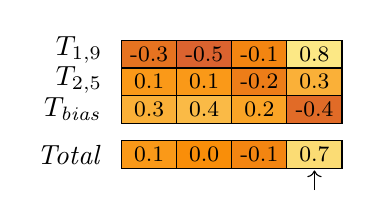
\begin{tikzpicture}
		% Top half
		\def\topacs{
			{-0.3,-0.5,-0.1,0.8},
			{0.1,0.1,-0.2,0.3},
			{0.3,0.4,0.2,-0.4}%
		}
		
		\foreach \line [count=\y] in \topacs {
			\foreach \pix [count=\x] in \line {
				\ifthenelse{\lengthtest{\pix pt < 0 pt}}{
					\pgfmathtruncatemacro\lambda{(\pix+1)*100}
					\draw[shift={(-0.7,0)},fill=midac!\lambda!lowac] (0.7*\x,-0.35*\y) rectangle +(0.7,0.35);
				}{
					\pgfmathtruncatemacro\lambda{\pix*100}
					\draw[shift={(-0.7,0)},fill=highac!\lambda!midac] (0.7*\x,-0.35*\y) rectangle +(0.7,0.35);
				}
				\node[shift={(-0.35,0.175)}] at (0.7*\x,-0.35*\y) {\footnotesize \pix};
			}
		}
		
		\draw[xstep=0.7cm,ystep=0.35cm,shift={(0,0)}] (0,-1.06) grid (2.8,0);
		\node[label=left:{$T_{1,9}$},shift={(0,-0.125)}] at (0,0) {}; 
		\node[label=left:{$T_{2,5}$},shift={(0,-0.125)}] at (0,-0.375) {}; 
		\node[label=left:{$T_{\mathit{bias}}$},shift={(0,-0.125)}] at (0,-0.75) {};
		
		% bottom half
		\def\botacs{
			{0.1,0.0,-0.1,0.7}%
		}
		
		\foreach \line [count=\y] in \botacs {
			\foreach \pix [count=\x] in \line {
				\ifthenelse{\lengthtest{\pix pt < 0 pt}}{
					\pgfmathtruncatemacro\lambda{(\pix+1)*100}
					\draw[shift={(-0.7,-1.275)},fill=midac!\lambda!lowac] (0.7*\x,-0.35*\y) rectangle +(0.7,0.35);
				}{
					\pgfmathtruncatemacro\lambda{\pix*100}
					\draw[shift={(-0.7,-1.275)},fill=highac!\lambda!midac] (0.7*\x,-0.35*\y) rectangle +(0.7,0.35);
				}
				\node[shift={(-0.35,-1.1)}] at (0.7*\x,-0.35*\y) {\footnotesize \pix};
			}
		}
		
		\draw[xstep=0.7cm,ystep=0.35cm,shift={(0,-1.275)}] (0,-0.35) grid (2.8,0);
		\node[label=left:{$\mathit{Total}$},shift={(0,-0.175)}] at (0,-1.275) {};
		
		\draw [->] (2.45, -1.9) -- (2.45, -1.65);
		\end{tikzpicture}
	}
	\caption{\centering Value Estimation and Action Selection\label{fig:tilecode-select}}
\end{subfigure}

\caption{
	State-action value approximation, when tile coding used.
	\label{fig:tilecode}
}
\end{figure}
\end{frame}

\begin{frame}{Reinforcement Learning: An Example (II)}
\begin{figure}
	\centering
	\resizebox{0.5\linewidth}{!}{
		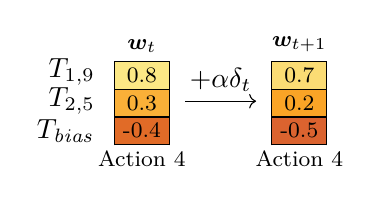
\begin{tikzpicture}		
		% Top half
		\def\startacs{
			{0.8},
			{0.3},
			{-0.4}%
		}
		
		\foreach \line [count=\y] in \startacs {
			\foreach \pix [count=\x] in \line {
				\ifthenelse{\lengthtest{\pix pt < 0 pt}}{
					\pgfmathtruncatemacro\lambda{(\pix+1)*100}
					\draw[shift={(-0.7,0)},fill=midac!\lambda!lowac] (0.7*\x,-0.35*\y) rectangle +(0.7,0.35);
				}{
					\pgfmathtruncatemacro\lambda{\pix*100}
					\draw[shift={(-0.7,0)},fill=highac!\lambda!midac] (0.7*\x,-0.35*\y) rectangle +(0.7,0.35);
				}
				\node[shift={(-0.35,0.175)}] at (0.7*\x,-0.35*\y) {\footnotesize \pix};
			}
		}
		
		\draw[xstep=0.7cm,ystep=0.35cm,shift={(0,0)}] (0,-1.06) grid (0.7,0);
		\node[label=left:{$T_{1,9}$},shift={(0,-0.125)}] at (0,0) {}; 
		\node[label=left:{$T_{2,5}$},shift={(0,-0.125)}] at (0,-0.375) {}; 
		\node[label=left:{$T_{\mathit{bias}}$},shift={(0,-0.125)}] at (0,-0.75) {};
		\node[label=below:{\footnotesize Action 4},shift={(0.35,-0.125)}] at (0,-0.75) {};
		\node[label=above:{\footnotesize $\wvec{t}$},shift={(0.35,-0.125)}] at (0,0) {};
		
		\def\finalacs{
			{0.7},
			{0.2},
			{-0.5}%
		}
		
		\foreach \line [count=\y] in \finalacs {
			\foreach \pix [count=\x] in \line {
				\ifthenelse{\lengthtest{\pix pt < 0 pt}}{
					\pgfmathtruncatemacro\lambda{(\pix+1)*100}
					\draw[shift={(2-0.7,0)},fill=midac!\lambda!lowac] (0.7*\x,-0.35*\y) rectangle +(0.7,0.35);
				}{
					\pgfmathtruncatemacro\lambda{\pix*100}
					\draw[shift={(2-0.7,0)},fill=highac!\lambda!midac] (0.7*\x,-0.35*\y) rectangle +(0.7,0.35);
				}
				\node[shift={(2-0.35,0.175)}] at (0.7*\x,-0.35*\y) {\footnotesize \pix};
			}
		}
		
		\draw[xstep=0.7cm,ystep=0.35cm,shift={(2,0)}] (0,-1.06) grid +(0.7,1.06);
		\node[label=below:{\footnotesize Action 4},shift={(2.35,-0.125)}] at (0,-0.75) {};
		\node[label=above:{\footnotesize $\wvec{t+1}$},shift={(0.35,-0.125)}] at (2,0) {};
		
		\draw[->] (0.9,-0.5) -- node[above] {$+ \alpha \delta_t$} (1.8,-0.5);
		\end{tikzpicture}
	}
	
	\caption{
		Update step, for observed TD error $\delta_t=-0.2$ and $\alpha=0.5$.
		\label{fig:tilecode-update}
	}
\end{figure}
\end{frame}

\begin{frame}{Reinforcement Learning: An Example (III)}
\begin{figure}
	\centering
		\resizebox{0.9\linewidth}{!}{
			\begin{tikzpicture}
			\node at (0.0,-1.2){$s = \begin{pmatrix}
				0.7 \\
				0.3
				\end{pmatrix}$};
			\node at (0,-2.7) {$\bm{x}(s,\cdot) = \bm{x}'(s,\cdot)+\!\!\!\!+ \bm{x}''(s,\cdot)$};
%			\node at (0,-1.1) {$\bm{x}(s,\cdot) = \begin{Bmatrix}
%				T_{1,9}, \\
%				T_{2,5}, \\
%				T_{\mathit{bias}}
%				\end{Bmatrix}$};
			
			\node at (5.5,-0.5) {
				\begin{tikzpicture}
				\draw[xstep=1.5cm,ystep=0.25cm,color=uofgcobalt,opacity=0.7,shift={(-0.25,-0.5)},label=above:{Tiling 0}] (0,0) grid (1.5,1.5);
				\fill[uofgcobalt,opacity=0.5,] (-0.25,-0.25) rectangle (1.25,0);
				\node[color=uofgcobalt] at (0,1.15) {\footnotesize Tiling 1};
				
%				\draw[step=0.5cm,color=uofgpumpkin,opacity=0.7,shift={(0.25,-0.25)},label=above:{Tiling 1}] (-0.5,-0.5) grid (1,1);
				\draw[xstep=1.5cm,ystep=0.25cm,color=uofgpumpkin,opacity=0.7,shift={(-0.25,-0.83)},label=above:{Tiling 0}] (0,0) grid (1.5,1.5);
%				\fill[uofgpumpkin,opacity=0.5,shift={(0.25,-0.25)}] (0,0) rectangle (0.5,0.5);
				\fill[uofgpumpkin,opacity=0.5,] (-0.25,-0.33) rectangle (1.25,-0.08);
				\node[color=uofgpumpkin] at (0.25,-1.05) {\footnotesize Tiling 2};
				
				\node[circle, black, draw,
				fill, radius=0.5pt, inner sep=0pt,minimum size=1.5pt, label=above:{$s$}] at (0.625,-0.125) {};
				%			\filldraw (0.625,-0.125) circle[radius=1.5pt,label=above:{$s$}];
				
				\draw[->] (-0.25,-0.5)--(-0.25,0.85);
				\draw[->] (-0.25,-0.5)--(1.1,-0.5);
				
				\node at (1,-0.7) {\footnotesize 1};
				\node at (-0.4,0.75) {\footnotesize 1};
				\node at (-0.35,-0.6) {\footnotesize 0};
				
				\node at (3,0) {$\bm{x}'(s,\cdot) = \begin{Bmatrix}
					T_{1,5}, \\
					T_{2,4}
					\end{Bmatrix}$};
				\end{tikzpicture}
			};
		
		\node at (5.5,-3) {
			\begin{tikzpicture}
			\draw[xstep=0.75cm,ystep=1.5cm,color=uofglavendar,opacity=0.7,shift={(-0.5,-0.5)},label=above:{Tiling 0}] (0,0) grid (1.5,1.5);
			\fill[uofglavendar,opacity=0.5,] (0.25,-0.5) rectangle (1,1);
			\node[color=uofglavendar] at (0,1.15) {\footnotesize Tiling 3};
			
			\draw[xstep=0.75cm,ystep=1.5cm,color=uofglawn,opacity=0.7,shift={(-0.1,-0.5)},label=above:{Tiling 0}] (0,0) grid (1.5,1.5);
			\fill[uofglawn,opacity=0.5,] (-0.10,-0.5) rectangle (0.65,1);
			\node[color=uofglawn] at (1,-1) {\footnotesize Tiling 4};
			
			\node[circle, black, draw,
			fill, radius=0.5pt, inner sep=0pt,minimum size=1.5pt, label=above:{$s$}] at (0.625,-0.125) {};
			%			\filldraw (0.625,-0.125) circle[radius=1.5pt,label=above:{$s$}];
			
			\draw[->] (-0.25,-0.5)--(-0.25,0.85);
			\draw[->] (-0.25,-0.5)--(1.1,-0.5);
			
			\node at (1,-0.7) {\footnotesize 1};
			\node at (-0.4,0.75) {\footnotesize 1};
			\node at (-0.35,-0.6) {\footnotesize 0};
			\node at (3,0) {$\bm{x}''(s,\cdot) = \begin{Bmatrix}
				T_{3,2}, \\
				T_{4,1}
				\end{Bmatrix}$};
			\end{tikzpicture}
		};
			
		\end{tikzpicture}
	}

\caption{
	Other codings.
	\label{fig:tilecode-varied}
}
\end{figure}
\end{frame}

\begin{frame}{Where has RL succeeded in networks?}
	%Link to recent work in data-driven networking/optimisation?
	%
	%Link to that one GMM paper w/ RL communication.
	
	\begin{itemize}
		\item \alert{Data-driven networking.} Effectively applied to intra-domain routing \footcite{DBLP:conf/hotnets/ValadarskySST17}, task allocation \footcite{DBLP:conf/hotnets/MaoAMK16}, traffic optimisation \footcite{DBLP:conf/sigcomm/ChenL0L18}, video adaptive bitrate selection \footcite{DBLP:conf/sigcomm/MaoNA17} and more, each with general and domain-specific insights.
		
		\item \alert{In anomaly detection?} Optimising information sharing in distributed statistical model training \footcite{DBLP:conf/paisi/XuSH07}.
	\end{itemize}
\end{frame}

%\begin{frame}{What might we gain from RL in DDoS prevention?}
%content...
%\end{frame}

%\section{Existing work}

\section{The limits of existing work}

\begin{frame}{Multiagent RL (MARL) for DDoS prevention}
%	Network Model \footcite{DBLP:journals/eaai/MalialisK15}
%	
%	Pushback \footcite{DBLP:journals/ccr/MahajanBFIPS02a}
%	
%	Group reward functions etc.
%
%	Its weaknesses? Strong assumptions about what knowledge the learners really have...
	
	\begin{itemize}
		\item There are existing RL-based DDoS defences like MARL\footcite{DBLP:journals/eaai/MalialisK15}.
		% How? Violation of ISP-like criterion, 
		
		\item Network model
		\begin{itemize}
			\item Hosts have a fixed probability of being benign/malicious.
			\item Tree overlay topology (split into teams) protecting one server.
			\item Per-team rewards: \alert{coordinated team learning}.
			\item Action: (per-timestep) choose $p\in\{0,10,...,90\}$, s.t. each learner (egress/ingress switch) drops $p\%$ of inbound traffic.
		\end{itemize}
	
%		\item Implemented in mininet with Ryu controller, traffic generated by replaying traces.
%		\begin{itemize}
%			\item Packet content unimportant---only need accurate load stats/queuing behaviour.
%			\item Alternate model featuring live HTTP traffic.
%		\end{itemize}
	\end{itemize}
\end{frame}

\begin{frame}{Multiagent RL (MARL) for DDoS prevention}
\begin{columns}
	\begin{column}{0.45\linewidth}
		\begin{itemize}
			\item Algorithm: Semi-gradient Sarsa, linear fn approx, $\epsilon$-greedy selection.
			\item Actions: Drop [0, 10, ... 90]\si{\percent} upstream traffic.
			\item State: load vectors of agent and parents ($\mathbb{R}^4$) $\rightarrow$ tile-coded.
			\item Rewards: \num{-1} if $\mathit{load} > U_s$, else fraction of surviving legit traffic.
		\end{itemize}
	\end{column}
	\begin{column}{0.5\linewidth}
		\begin{figure}
			\centering
			\resizebox{\linewidth}{!}{
				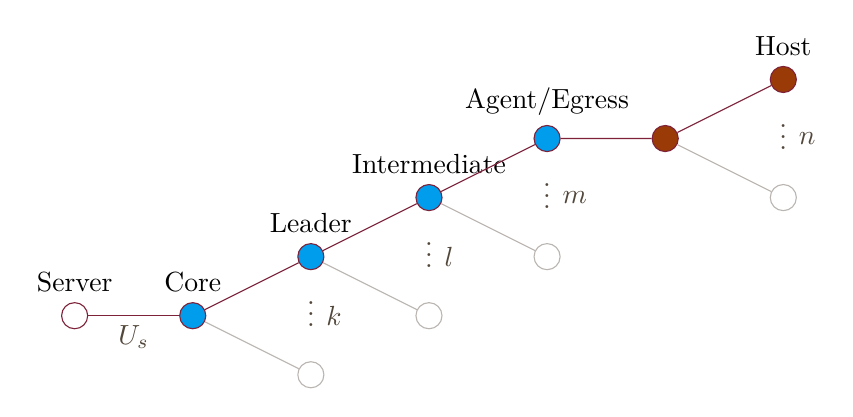
\begin{tikzpicture}[
				texts/.style = {text=black},
				labeltexts/.style = {text=uofgsandstone},
				treeline/.style = {draw=uofgburgundy},
				treenode/.style = {texts, circle, centered, fill=white, treeline},
				load/.style = {fill=uofgcobalt},
				external/.style = {fill=uofgrust},
				hideline/.style = {draw=uofgsandstone!40!white},
				hidenode/.style = {treenode, hideline},
				grow'=right
				]
				\node[treenode, label={[texts]above:Server}] (root) {}
				child [treeline] { node [treenode, load, label={[texts]above:Core}] (sswitch) {}
					child [treeline] { node [treenode, load, label={[texts]above:Leader}] (teaml) {} 
						child [treeline] { node [treenode, load, label={[texts]above:Intermediate}] (inter) {}
							child [treeline] { node [treenode, load, label={[texts]above:Agent/Egress}] (agent) {}
								child [treeline] { node [treenode, external] (extern) {}
									child [treeline] { node [treenode, external, label={[texts]above:Host}] (host) {} }
									child [hideline] { node [hidenode] (endhost) {} }
								}
							}
							child [hideline] { node [hidenode] (endagent) {} }
						}
						child [hideline] { node [hidenode] (endinter) {} }
					}
					child [hideline] { node [hidenode] (endteaml) {} }
					edge from parent
					node[below, labeltexts] {$U_s$}
				};
				
				%\draw[-] (teaml) -- (endteaml);
				\node [labeltexts] (kdots) at ($(teaml)!0.5!(endteaml)$) {$\rvdots$};
				\node [labeltexts, right = -0.1cm of kdots] {$k$};
				\node [labeltexts] (ldots) at ($(inter)!0.5!(endinter)$) {$\rvdots$};
				\node [labeltexts, right = -0.1cm of ldots] {$l$};
				\node [labeltexts] (mdots) at ($(agent)!0.5!(endagent)$) {$\rvdots$};
				\node [labeltexts, right = -0.1cm of mdots] {$m$};
				\node [labeltexts] (ndots) at ($(host)!0.5!(endhost)$) {$\rvdots$};
				\node [labeltexts, right = -0.1cm of ndots] {$n$};
				\end{tikzpicture}
			}
			\caption{
				Network topology diagram.
				Red nodes are external, blue nodes feature in the state vector.
				Any packet drop occurs when forwarding packets from an egress switch to its parent (intermediate) switch.
			}
		\end{figure}
	\end{column}
\end{columns}
\end{frame}

\begin{frame}{Multiagent RL (MARL) for DDoS prevention}
%	Network Model \footcite{DBLP:journals/eaai/MalialisK15}
%	
%	Pushback \footcite{DBLP:journals/ccr/MahajanBFIPS02a}
%	
%	Group reward functions etc.
%
%	Its weaknesses? Strong assumptions about what knowledge the learners really have...

\begin{itemize}
	\item Yet existing RL-based DDoS defences like MARL haven't been successful---why?
	
	\item \alert{Actions not granular}---many hosts punished accidentally.
	\item \alert{Action affects congestion-aware traffic disproportionately}---TCP, QUIC \emph{actively slow down} if packets lost.
\end{itemize}
\end{frame}

%\begin{frame}{The case for finer granularity}
%	\begin{columns}
%	\begin{column}{0.45\linewidth}
%		\begin{itemize}
%			\item Learner/host ratio (action/host ratio) affects host QoS.
%			
%			\item Reduced service guarantees by nature of \emph{pushback} model.
%			\begin{itemize}
%				\item \alert{Worse with good-faith TCP congestion avoidance}.
%			\end{itemize}
%			%This is exacerbated by TCP congestion avoidance---legit hosts will be punished far more severely, bad actors don't care!
%			
%%			\item More granular $\implies$ should focus on flow stats, \alert{not aggregates} like now! %Alongside this higher-granularity view, reformulation to include flow characteristics in the decision-making process.
%		\end{itemize}
%	\end{column}
%	\begin{column}{0.5\linewidth}
%		\begin{figure}
%			\includegraphics[width=\linewidth]{../plots/online-varyN-binary-pres.pdf}
%			\caption{Service quality decreases as actions become less granular (affecting $n$ hosts at once).}
%		\end{figure}
%	\end{column}
%	\end{columns}
%\end{frame}
%
%\begin{frame}{The case for finer granularity}
%\centering
%\includegraphics[width=0.8\linewidth]{../plots/online-varyN-binary-pres.pdf}
%\end{frame}

\begin{frame}{Why care about congestion-aware traffic?}
\begin{columns}
	\begin{column}{0.5\linewidth}
		\begin{figure}
			\includegraphics[width=\linewidth]{../code/caida-stats/plots/ca-monthly-pres-bytes.pdf}
			\caption{Proportion of traffic volume which is congestion aware (TCP or QUIC) (CAIDA 2018 passive trace dataset).}
		\end{figure}
	\end{column}
	\begin{column}{0.45\linewidth}
		\begin{itemize}
			\item 9 years ago, TCP carried \SIrange{89}{98}{\percent} of data by volume\footnotemark.
			\item Nowadays, CAIDA traces suggest \SIrange{75}{84}{\percent} over both directions of a backbone link. If we include QUIC, \SIrange{76}{85}{\percent}.
			\item QUIC is a non-negligible fraction (peak \SI{4.5}{\percent} Dir A in Jul/Sep), and we can't examine anything below headers.
		\end{itemize}
	\end{column}
\end{columns}
\footcitetext{DBLP:conf/saint/ZhangDJC09}
\end{frame}

\begin{frame}{Why care about congestion-aware traffic?}
\centering
\includegraphics[width=0.8\linewidth]{../code/caida-stats/plots/ca-monthly-pres-bytes.pdf}
\end{frame}

%\begin{frame}{And the replication reveals...}	
%\begin{itemize}
%	\item Network topology has no basis in reality---admitted by its \emph{own} source work \footcite{DBLP:journals/ccr/MahajanBFIPS02a}.
%	
%	\item Action granularity causes more collateral damage than we'd like...
%	
%	\item ...and the picture is worse still for legitimate TCP flows.
%	
%	\item Reward function needs a priori knowledge/reliable estimates to learn online.
%	
%	\item \alert{But on the plus side, action computation is fast: \SIrange{80}{100}{\micro\second}.}
%\end{itemize}
%\end{frame}
%
%\begin{frame}{How can we use these observations? (The Immediate Future)}
%\begin{itemize}
%	\item \textbf{\alert{Why not take actions on a per-flow basis?}}
%	\begin{itemize}
%		\item Solves the granularity issues by construction.
%		\item Allows different treatment by flow features (i.e., protocol).
%	\end{itemize}
%	\item Need to rethink state space: more costly computation, but we have room to work in.
%	\begin{itemize}
%		\item We need any additions to be justified beyond just ``more data'', since \alert{changes affect training time and execution time}.
%	\end{itemize}
%	\item How do we select flows to act upon?
%\end{itemize}
%\end{frame}

\section{How do we adapt MARL to match the realities of network traffic?}

\begin{frame}{Adapting MARL}
\begin{itemize}
	\item Prior work with these techniques has two key flaws:
	\begin{itemize}
		\item Each action can (and will!) map to many flows (particularly in real networks), increasing the \alert{likelihood} of collateral damage.
		\item The majority of internet traffic is congestion-aware, increasing the \alert{cost} of collateral damage.
	\end{itemize}
	\item Naturally, we aim then to take decisions \emph{per-flow} (or per-source, to be precise).
\end{itemize}
\end{frame}

\begin{frame}{Network Model}
\begin{itemize}
	\item \textbf{Topology}: Identical to MARL's ``online'' experiments (single server, $k=2, \ell=3, m=2, \operatorname{P}_{\mathit{malicious}}=0.4$), but varying $n \in \{2, 4, 8, 16\}$.
	\begin{itemize}
		\item \numrange{24}{192} hosts, causing expected bandwidth load \SIrange{2.03}{2.18}{$\! \times U_s$}.
	\end{itemize}
	\item \textbf{TCP Traffic}: HTTP traffic (\emph{nginx} and \emph{libcurl}), random requests (long and short flows), TCP Cubic.
	\item \textbf{UDP Traffic (Malicious/Benign)}: \emph{hping3}, MTU-size packets (mapping to an amplification attack).
\end{itemize}
\end{frame}

\begin{frame}{An effective state space}
\begin{itemize}
	\item \textbf{Global state} The existing state space (load measurements).
	\item \textbf{Constants} Source IP.
	\item \textbf{Ongoing observations} Flow duration, flow size, packets in/out, correspondence ratio, mean inter-arrival time.
	\item \textbf{Per-timestep (window) observations} Last action taken, $\mathbf{\Delta}$ send/receive rate, mean packet size, packet in/out count.
\end{itemize}

	Why exclude port numbers, payload features? \alert{QUIC} and similar protocols \emph{will become ubiquitous}. \alert{This constraint is a form of protocol-agnostic future-proofing}.

%	Tile code each feature individually.
\end{frame}

\begin{frame}{Feature Performance---UDP}
\begin{figure}
	\centering
	\includegraphics[width=0.8\linewidth]{../plots/ftprep-box-pres}
%	\vspace{-1.2cm}
	\caption{
		Learned performance of Marl++ agents when benign traffic is UDP-like, using only a single feature as a basis for decisions. Uncap.
		\label{fig:udp-feature-plots}
	}
\end{figure}
\end{frame}

\begin{frame}{Feature Performance---TCP}
\begin{figure}
	\centering
	\includegraphics[width=0.8\linewidth]{../plots/ftprep-tcp-cap-box-pres}
%	\vspace{-1.2cm}
	\caption{
		Learned performance of Marl++ agents when benign traffic is TCP-like, using only a single feature as a basis for decisions.
		\label{fig:udp-feature-plots-cap}
	}
\end{figure}
\end{frame}

\begin{frame}{Implementation considerations}
	\begin{itemize}
		\item \alert{Timed random sequential decisions}
		\begin{itemize}
			\item Multiple actions per timestep---perform up to a deadline of \SI{1}{\milli\second} as suggested\footcite{DBLP:conf/sigcomm/ChenL0L18}.
			\item Carry over undone work to next timestep, fuse window measurements.
			\item Optionally drop after a few rounds to prevent starvation.
		\end{itemize}
		\item Reward functions modified for direction awareness.
		\item Optional model updates from other agents' traces/experience.
		\item Deliberately avoiding neural networks; training time, execution cost, energy usage, hardware...
		\item I'll refer to all these advancements with MARL-like actions as \alert{MARL++}.
	\end{itemize}
\end{frame}

\begin{frame}{Another look at actions---SPF}
\begin{itemize}
	\item Behavioural knowledge---SPIFFY\footcite{DBLP:conf/ndss/KangGS16} realised that \alert{volume-based attack flows can't scale up if they have their maximum bandwidth increased}.
	\item Can we constrain our model to speed up training/reduce variance?
	\item Limit $p \in \left\{ 0.00, 0.05, 0.25, 0.50, 1.0 \right\}$, can only increase/decrease one step at a time.
	\begin{itemize}
		\item All flows start at $p = 0.05$.
	\end{itemize}
	\item \alert{3 actions}---\emph{punish, reward, no-op}.
	\item Now need us to choose $\gamma$ to \emph{plan ahead}: 0.8 an effective choice.
\end{itemize}
\end{frame}

\section{Evaluation}
\begin{frame}{UDP traffic performance}
\begin{columns}
	\begin{column}{0.7\linewidth}
	\begin{figure}
		\centering
		\includegraphics[width=0.95\linewidth]{../plots/udp-box-pres}
		
		\caption{
			Online performance for UDP-like benign traffic.
			\label{fig:udp-box}
		}
	\end{figure}
	\end{column}
	\begin{column}{0.3\linewidth}
		\begin{itemize}
			\item Marl++ outperforms Marl---a success!
			\item SPF has low variance as expected, but performs poorly until large $n$.
		\end{itemize}
	\end{column}
\end{columns}
\end{frame}

\begin{frame}{TCP traffic performance}
\begin{columns}
	\begin{column}{0.3\linewidth}
		\begin{itemize}
			\item Harder to see statistically significant advantage until large $n$.
			\item All have very high variance (due to poor actions on congestion-aware protocols), but SPF narrows it down.
		\end{itemize}
	\end{column}
	\begin{column}{0.7\linewidth}
		\begin{figure}
			\centering
			\includegraphics[width=0.95\linewidth]{../plots/tcp-box-pres}
			
			\caption{
				Online performance for UDP-like benign traffic.
				\label{fig:tcp-box}
			}
		\end{figure}
	\end{column}
\end{columns}
\end{frame}

\begin{frame}{TCP traffic (n=16)---training in detail}
	\begin{figure}
		\centering
		\includegraphics[width=0.8\linewidth]{../plots/tcp-16-single-pres}
		
		\caption{
			Online performance of standard and single-agent models with $n=16$ hosts per egress point and TCP-like benign traffic.
			At this level of host density, SPF reaches its peak performance sooner and is considerably more consistent throughout the episode.
			Marl++ takes longer to reach its most effective policy, and achieves visibly better peak performance than the other standard models.
			With a single agent, Marl++ shows worse performance, while SPF improves significantly and continues to learn well past annealing $\epsilon \rightarrow 0$.
			\label{fig:tcp-16}
		}
	\end{figure}
\end{frame}

\begin{frame}{All experiments}
	\begin{table}
		\centering
		\resizebox{\linewidth}{!}{\expandableinput ../tables/big-avg-reward.tex}
		\caption{Average reward for combinations of model, host density and traffic class.\label{tab:av-vals}}
	\end{table}
\end{frame}

\begin{frame}{Main take-homes}
\begin{itemize}
	\item The flow-level focus \alert{improves over past RL work in both problem cases}.
	\begin{itemize}
		\item Still a long way to go before it's competitive with established solutions.
		\item Likely converging to, and becoming stuck in, locally optimal (but globally sub-optimal) policies.
	\end{itemize}
	\item SPF relies on higher volumes of data to perform well (high $n$, experience sharing)---has potential to be useful if this need can be met.
	\begin{itemize}
		\item Why?
	\end{itemize}
\end{itemize}
\end{frame}

\section{The work yet undone}

\begin{frame}{Other environments}
\begin{itemize}
	\item Expansion to other topologies.
	\begin{itemize}
		\item Likely not viable or sensible to map this overlay topology to most networks: many sources/sinks, multiple paths make global state useless.
		\item \alert{Then what we need to change is global state!}
	\end{itemize}
	\item So flip the problem on its head: even in multipath networks \emph{we know what path a flow will follow} (i.e., via ECMP).
	\begin{itemize}
		\item So, draw global state from the \emph{path}: endpoints + tertiles (still in $\mathbb{R}^{4}$).
		\item Cost: possibly more network measurements, concept of teams no longer valid (so lose info from reward functions).
	\end{itemize}
	\item This will enable direct comparison against other approaches.
\end{itemize}
\end{frame}

\begin{frame}{Other attacks}
\begin{itemize}
	\item More ``old-school'' attacks like TCP SYN/ACK floods, application-level attacks against emulated software...
	\item In AS-like networks/topologies, we can examine \alert{Link Flooding Attacks}.
	\item Crucially, need several of these to evaluate against attackers with \alert{evolving strategies} (and show generalisation beyond amplification attacks).
	\begin{itemize}
		\item Evolving attackers are \emph{the norm}\footcite{DBLP:conf/spw/KangGS16}, though few works detail \emph{how} they evolve.
	\end{itemize}
\end{itemize}
\end{frame}

\begin{frame}{The Near Future}
\begin{itemize}
	\item Reward functions without dependence on ahead-of-time knowledge.
	\begin{itemize}
		\item I.e., for certain distributions of communication we might want to maximise link utilisation in both directions.
		\item Active measurement---canary flows etc.
	\end{itemize}

\item Deriving normal model behaviour from traces.
\begin{itemize}
	\item We only need to simulate specific behaviour to test these enhancements, but that can become more representative.
	\item But we do need more diversity of services in the normal model.
\end{itemize}

\item Investigate other RL algorithms.
\begin{itemize}
	\item ``Deep learning'' probably not feasible.
	\item \alert{$\operatorname{TD}(\lambda)$, actor-critic methods}.
\end{itemize}
\end{itemize}
\end{frame}

\begin{frame}{The Far Future}
\begin{itemize}
	\item Other problems.
	\begin{itemize}
		\item New action spaces, careful consideration.
	\end{itemize}
\item Adversarial capabilities---evasion and poisoning attacks.
\item Knowledge-sharing between agents: cost-modelling and optimisation.
\item Test deployments in real networks.
\end{itemize}
\end{frame}

\begin{frame}[standout]{Conclusion}
	We've looked at...
	\begin{itemize}
		\item A quick introduction to RL, and its \alert{importance to future networks}.
		\item A recent `direct control' approach to intrusion prevention, and \alert{its significant weaknesses}.
		\item A \alert{new interaction model and state-space}, which can remedy these weaknesses.
		\item The \alert{next steps} towards proper generalisation.
	\end{itemize}
	
	\alert{Questions?}
\end{frame}

\appendix

\begin{frame}[allowframebreaks]{References}
\printbibliography[heading=none]
\end{frame}

\end{document}
